\documentclass[12pt,french,twoside]{exam}
\noprintanswers 

\input{../../../../Preambule/LesIndispensables}
\input{../../../../Preambule/MesDS}

\begin{document}

%%%%%%%%%%%%%%%%%%%% En-tête etc %%%%%%%%%%%%%%%%%%%

\runningheader{}{}{DS \no ...   } %%%%%%%%%%%% à compléter 
\tikzset{Bloc/.style={rectangle, draw, minimum height=10mm}}

\begin{center}
{\setlength{\fboxrule}{0.3mm}
\fbox{\begin{minipage}{18.5cm}{\begin{center}\vspace{0.2cm}
%%%%%%%%%% le numéro du DS 
{\LARGE \textbf{Devoir Surveillé \no ...}} \\ %%%%%%%%%%%% à compléter 
\vspace{0.5cm}
\begin{Large}
%%%%%%%%%% le titre du DS 
\textbf{    } %%%%%%%%%%%% à modifier 
\end{Large}
\vspace{0.2cm}
\begin{flushright}
%%%%%%%%%% la date du DS 
{\large \textit{...}} %%%%%%%%%%%% à compléter 
\end{flushright}
\end{center}}\end{minipage}}}
\end{center}
\vspace{0.2cm}
\begin{tcolorbox}[title = Quelques consignes]
Le candidat attachera la plus grande importance à la clarté, à la précision et à la concision de la rédaction. Si un candidat est amené à repérer ce qui peut lui sembler être une erreur d'énoncé, il le signalera sur sa copie et devra poursuivre sa composition en expliquant les raisons des initiatives qu'il a été amené à prendre.\\

Les trois exercices sont indépendants.
\end{tcolorbox}

%\vspace{0.8cm}
%\bigskip
%%%%%%%%%%%%%%%%%%%%% Le sujet %%%%%%%%%%%%%%%%%%%%


\part*{Piéger une particule}


\begin{multicols}{2}
\begin{center}
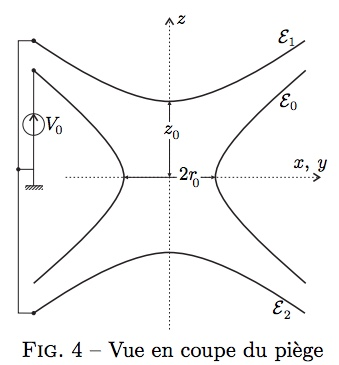
\includegraphics[scale=0.6]{piege.jpeg} 
\end{center}
L’objectif est de piéger une particule chargée en vue de la refroidir et la garder ainsi stockée le plus longtemps possible. L’idée la plus simple consiste à piéger cette particule dans un puits de potentiel. Le dispositif de piégeage est représenté sur la figure 4, il compte trois électrodes présentant une symétrie de révolution autour d’un axe $(Oz)$. La première, notée $\mathcal{E}_0$, est en forme d’anneau de rayon interne $r_0$ et d’équation $x^2 + y^2 - 2z^2 = r_0^2$ , elle est portée à un potentiel $V_0$ positif. Les deux autres, notées $\mathcal{E}_1$ et $\mathcal{E}_2$, sont en forme de coupelles et correspondent aux deux nappes de l’hyperboloïde d’équation $x^2 + y^2 - 2z^2 = -2z_0^2$ , elles sont reliées à la masse. La distance minimale entre les deux coupelles est telle que $2z_0 = \sqrt{2}r_0$. 
\end{multicols}

On note $V(x,y,z)$ le potentiel régnant dans le piège initialement vide de charge. Ce potentiel est donc tel que $V(0, 0, z_0) = 0$ d’une part et d’autre part si $x^2 + y^2 = r_0^2$  alors $V(x,y,0) = V_0$.\\


On admet que le potentiel s’écrit sous la forme $V(x,y,z) = \frac{V_0}{2} + \frac{V_0}{2r_0^2}(x^2 + y^2 - 2z^2)$. \\ 

On admet qu’une particule de charge $q$ placée dans le piège est soumise à une force conservative de la forme $\vv{F}=-\dfrac{qV_0}{r_0^2}(x\widehat{u_x} + y\widehat{u_y} - 2z\widehat{uz})$. \\ 

\begin{questions}
\item Montrer que le point $O(0,0,0)$ est un équilibre. En écrivant le principe fondamental de la dynamique montrer que cet équilibre est globalement instable quel que soit le signe de la charge placée dans ce potentiel.\\

Afin d’éliminer l’instabilité démontrée à la question précédente, une première solution est d’ajouter un champ magnétique uniforme $\vv*{B}{0}$ selon l'axe $\widehat{u_z}$ avec $B_0 = 1,0$ T autour du dispositif électrostatique. Le piège devient ainsi « une trappe de PENNING », le mérite de sa mise en \oe uvre concrète est du à H. G. DEHMELT qui reçut le prix Nobel de physique en 1989 pour cette réalisation, l’idée originale, de F. M. PENNING, datant de 1936.\\ 

\item La particule piégée dans la trappe de PENNING est un antiproton $\overline{p}$ de masse $m_p$ et de charge $q = -e$. Établir les équations différentielles vérifiées par les fonctions $z(t)$ et $\zeta(t) = x(t) + iy(t)$. On introduira les constantes $\omega_c=\dfrac{eB_0}{m_p}$  et $\omega_0=\sqrt{\dfrac{eV_0}{m_pr_0^2}}$ . L'antiproton est-il confiné selon l'axe $Oz$ ? On admet que les solutions de l'équation différentielle en $\zeta$ conduisent à un confinement de l'antiproton dans le plan $xy$ si et seulement si le discriminant $\Delta$ de l'équation caractéristique est négatif. Montrer alors qu’il existe un champ $B_{\text{min}}$, tel que l’ajout d’un champ $B_0 > B_{\text{min}}$ conduit bien au confinement de l’antiproton dans le plan $xy$. Calculer la valeur de $B_{\text{min}}$ pour un piège tel que $V_0 = 5,0$ V et $r_0 = 5,7$ mm.

\item Calculer la valeur numérique de $\omega_0$ et $\omega_c$ pour la trappe de PENNING considérée. On exprimera la forme générale de $\zeta$ sous la forme $\zeta(t) = A\e^{r_+t} + B\e^{r_-t}$ où $r_+$ et $r_-$ sont les racines complexes de l'équation caractéristique établie à la question précédente et $A$ et $B$ sont des constantes d'intégration que l'on ne cherchera pas à déterminer. Donner les expressions de $r_+$ et $r_-$ en fonction de $\omega_c$ et $\omega_0$. En déduire que le mouvement confiné de l’antiproton dans cette trappe est la composition d’un mouvement rapide et de deux mouvements plus lents. On donnera une estimation simple des pulsations de ces trois mouvements en fonction de $\omega_0$ et $\omega_c$. \\ 
\textit{Attention : on ne demande pas de déterminer explicitement ou entièrement l'expression de $x(t)$ ou de $y(t)$. }\\


%Dans l’expérience GBAR, 
La trappe de PENNING permet de confiner les antiprotons, dont l’énergie cinétique d’entrée est estimée à 5 MeV. Pour les applications suivantes il est nécessaire de les refroidir jusqu’à une énergie de l’ordre de 150 eV. On se pose donc la question de savoir si le mouvement oscillant des antiprotons dans la trappe permet ce refroidissement.\\ 

On admet que le mouvement oscillant de l’antiproton est la source d’un rayonnement qui va contribuer à diminuer son énergie mécanique. La source principale de ce rayonnement est assurée par l’accélération selon l’axe $Oz$. La puissance moyenne $\langle P_{\text{ray}}\rangle_{T_0}$  rayonnée par l’antiproton sur une période $T_0 = \dfrac{2\pi}{\omega_0\sqrt{2}}$ caractéristique de son mouvement sinusoïdal paramétré par $z(t)$ est donnée par la relation 
\begin{center}
$ \langle P_{\text{ray}}\rangle_{T_0} = \dfrac{\mu_0e^2}{6\pi c}\langle \ddot{z}^2\rangle_{T_0}$
\end{center}
\item Déterminer l’ordre de grandeur de la température absolue des antiprotons à l’entrée de la trappe. Montrer que le rayonnement qu’il émet conduit à une décroissance exponentielle de l’énergie mécanique de l’antiproton caractérisée par une constante de temps $\tau$ que l’on exprimera en fonction de $m_p$, $\mu_0$, $e$, $c$ et $\omega_0$. En déduire la nécessité de recourir à une méthode de refroidissement complémentaire. \\

Cette méthode non étudiée ici est une thermalisation par chocs élastiques sur un nuage d’électrons confinés dans la trappe.
\end{questions}

\end{document}
